\begin{figure*}[t]
    \centering
    \begin{subfigure}[b]{0.45\textwidth}
        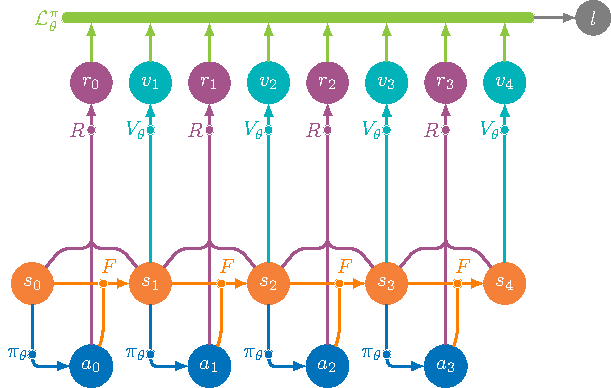
\includegraphics[width=\textwidth]{figs/shac.pdf}
        \caption{SHAC}
        \label{fig:shac}
    \end{subfigure}
    \begin{subfigure}[b]{0.45\textwidth}
        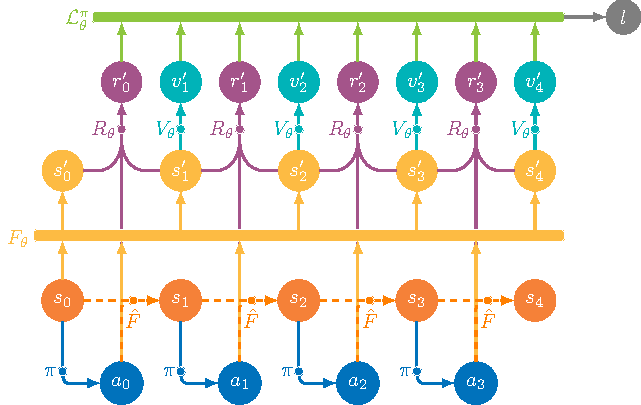
\includegraphics[width=\textwidth]{figs/shacpp.pdf}
        \caption{\fname{}}
        \label{fig:shacpp}
    \end{subfigure}
    \caption{Comparison between SHAC and \fname{}. Nodes with labels (such as $r_i$ or $r'_i$ represents values). Nodes without labels (such as $\pi$ or $R$) represents functions. Dashed lines are used to represent non differentiability}\label{fig:shac-shacpp}
\end{figure*}

\begin{algorithm}[t]
    \begin{algorithmic}[1]
    \STATE Initialize $\pi_\theta,V_\theta,R_\theta,F_\theta$ networks
    \STATE Initialize learning rates $\eta_\pi, \eta_R, \eta_V, \eta_F$
    \STATE Initialize environment $\mathcal{E}$
    \STATE Initialize $\gamma, \alpha$
    \FOR{episode in $1, \ldots, N_{\text{episodes}}$}
    
        
        \STATE $s,a,r,v \sim \mathcal{E}(\pi)$
        \STATE $\hat{s} = F_\theta(s_{:,0}, a)$
        \STATE $\hat{r} = R_\theta(\hat{s})$
        \STATE $\hat{v} = V_\theta(\hat{s})$
        
        \STATE $\theta \gets \theta - \eta_\pi \nabla \mathcal{L'}^\pi_\theta(\hat{r},\hat{v},\gamma,\alpha)$
        \STATE $\theta \gets \theta - \eta_V \nabla \mathcal{L}^V_\theta(\hat{v},s,v)$
        \STATE $\theta \gets \theta - \eta_R \nabla \mathcal{L}^R_\theta(\hat{r},s,a,r)$
        \STATE $\theta \gets \theta - \eta_F \nabla \mathcal{L}^F_\theta(\hat{s},s,a)$
    
    \ENDFOR
    
    \end{algorithmic}
    \caption{SHAC++ minimal (no cache and no cool-down) pseudocode. $s_{:,0}$ denotes the first step of each trajectory in $s$.}
    \label{alg:shacpp}
\end{algorithm}


\section{\fname{}}

As mentioned previously, we aim to address the limitations of SHAC by approximating the gradients of a differentiable environment ($R$ and $F$) with neural networks ($R_\theta$ and $F_\theta$). In particular, we aim to train a neural network to approximate the reward function by minimizing: 
$$ \mathbb{E}_{\tau\sim\pi}\left[\left|\left| \frac{1}{T}\sum_{i=0}^{T-1} R_{\theta}(s_i^\tau, a_i^\tau, s_{i+1}^\tau) - R(s_i^\tau, a_i^\tau, s_{i+1}^\tau) \right|\right|^2\right] $$

In practice, this is achieved by leveraging a \emph{replay buffer} to cache the state-action-reward triplets obtained from the environment. The neural network is then trained to minimize the mean squared error (MSE) loss. Specifically, we minimize the loss $\mathcal{L}_\theta^{R}:\mathcal{T}^N\rightarrow\mathbb{R}$:
$$ \mathcal{L}_\theta^R(B) = \frac{1}{N}\sum_{s,a,r \in B}\left|\left| R_\theta(s, a) - r \right|\right|^2 $$
Where $B$ represents a batch of state-action-reward triplets sampled uniformly from the cache.

Similarly, we aim to train a neural network to approximate the transition function. However, to avoid vanishing or exploding gradients, we employ a non-recursive approach similar similar to Action World Model~\cite{Ma24}. This corresponds to train a neural network that given a starting observation from $\mathcal{S}$ and a sequence of $H$ actions from $\mathcal{A}^H$, predicts the next $H$ observations from $\mathcal{S}^H$. We aim to minimize:

\begin{equation}
\begin{aligned}
\mathbb{E}_{\tau\sim\pi}\left[\frac{1}{NH}\sum_{t=0}^{T-H-1}\sum_{i=0}^{H-1} \left|\left| F_{\theta}(s_t^\tau, a_t^\tau, \dots, a_{t+H-1}^\tau)_i - \right.\right.\right. \\ \left.\left.\left. s_{t+i+1}^\tau \right|\right|^2\right] 
\end{aligned}
\end{equation}

In practice, this is achieved by caching trajectories and then training the neural network to minimize the MSE loss. That is, we minimize the loss $\mathcal{L}_\theta^{F}:\mathcal{T}^N\rightarrow\mathbb{R}$:
$$ \frac{1}{NH}\sum_{\tau \in B}\sum_{t=t_0}^{t_0+H-1}\left|\left| F_{\theta}(s_t^\tau, a_t^\tau, \dots, a_{t+H-1}^\tau)_i - s_{t+1}^\tau \right|\right|^2 $$
Where $B$ represents a batch of trajectories with horizon $H$ sampled uniformly from the cache.

Further, we modify the SHAC policy loss, $\mathcal{L}_\theta^{\pi}$, to include a term that penalizes actions outside the action space. That is, suppose the action space is $(a,b)$ (with $a<b$), we minimize the loss $\mathcal{L'}_\theta^\pi:$
\begin{figure*}[!t]
    \centering
    \begin{subfigure}[b]{0.24\textwidth}
        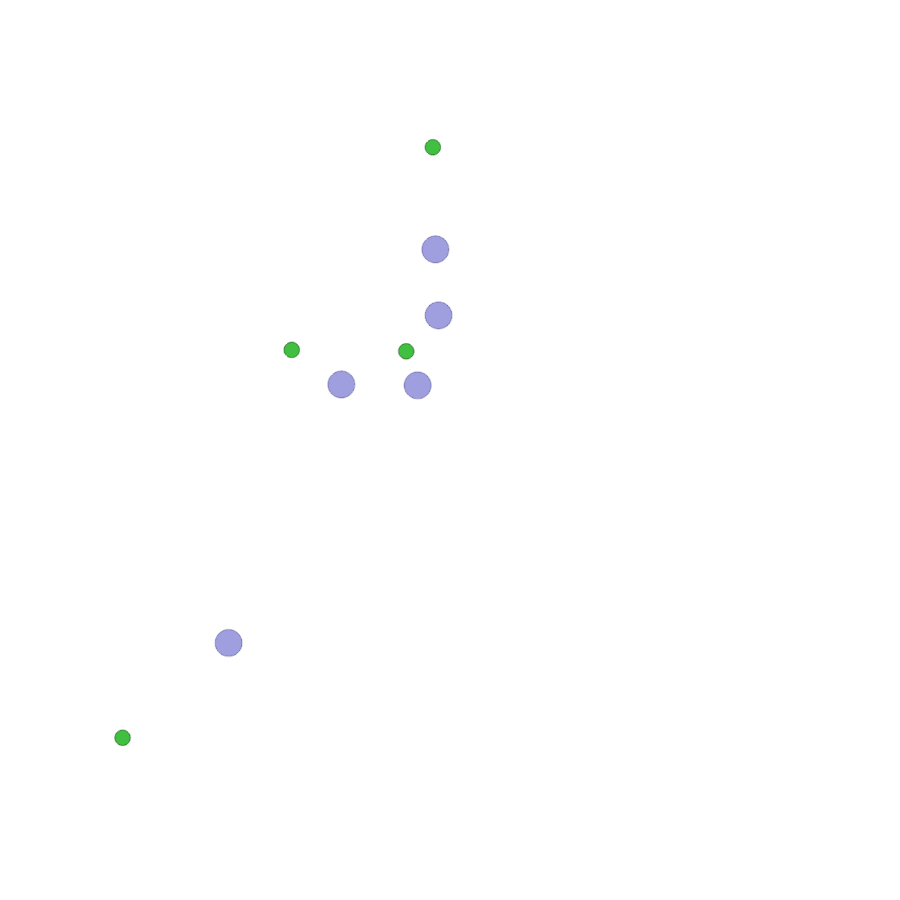
\includegraphics[width=\textwidth]{figs/dispersion.png}
        \caption{Dispersion}
        \label{fig:dispersion}
    \end{subfigure}
    \begin{subfigure}[b]{0.24\textwidth}
        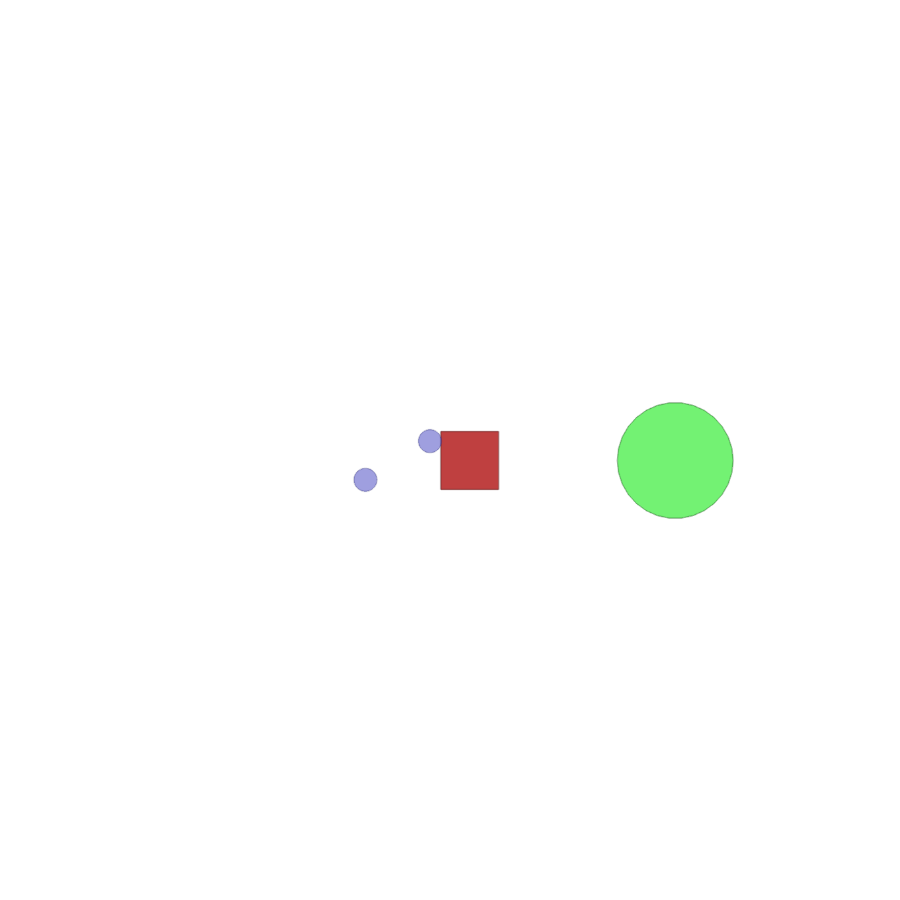
\includegraphics[width=\textwidth]{figs/transport.png}
        \caption{Transport}
        \label{fig:transport}
    \end{subfigure}
    \begin{subfigure}[b]{0.24\textwidth}
        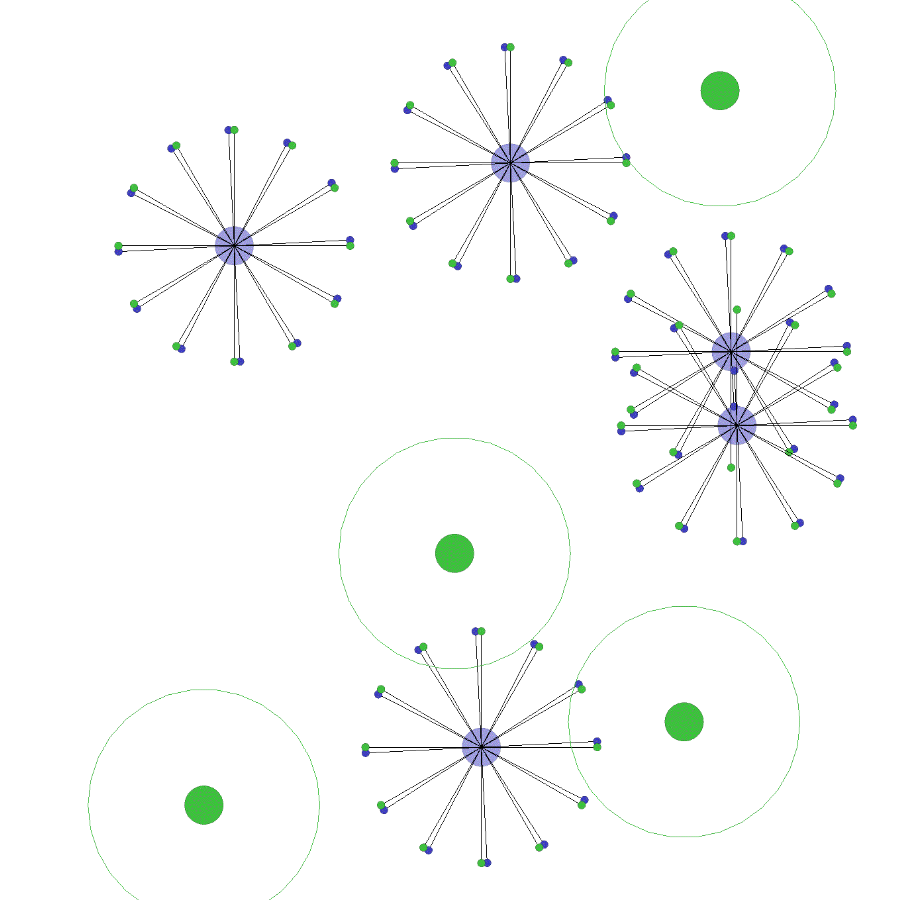
\includegraphics[width=\textwidth]{figs/discovery.png}
        \caption{Discovery}
        \label{fig:discovery}
    \end{subfigure}
    \begin{subfigure}[b]{0.24\textwidth}
        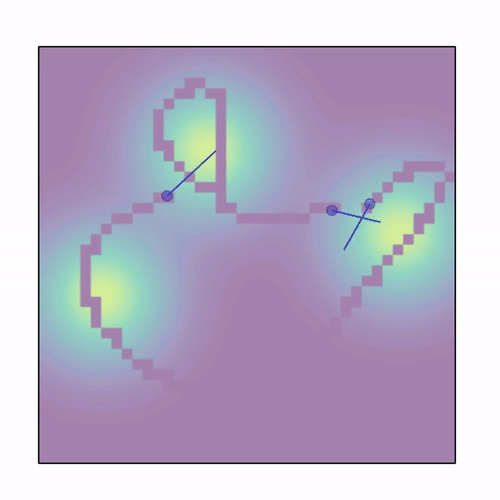
\includegraphics[width=\textwidth]{figs/sampling.png}
        \caption{Sampling}
        \label{fig:sampling}
    \end{subfigure}
    \caption{VMAS environments used in the experiments.}\label{fig:scenarios}
\end{figure*}

$$\mathcal{L}_\theta^\pi(B) + \alpha \frac{1}{NH}\sum_{\tau\in B}\sum_{t=t_0}^{t_0+H-1} d(a_t^\tau,(a,b))$$
$$d(x,(a,b)) = \begin{cases}(a-x)^2 & \text{if } x < a \\ (x-b)^2 & \text{if } x > b \\ 0 & \text{otherwise} \end{cases}$$

    Where $\alpha$ is a hyper-parameter that controls the strength of the penalty. In our experiments, we set $\alpha=1$. Usually, actions are either clipped to the allowed action space or, an activation function (such as hyperbolic tangent or sigmoid) is used to ensure that the actions are within the allowed range. While this approach is acceptable for algorithms like PPO and SHAC, the penalty we employ is crucial in our specific scenario. This necessity arises from the fact that we are training the policy to optimize two neural networks that serve as environment approximations. Because these networks are never trained with data outside the permissible action space, they are likely to be maximized beyond these bounds. Consequently, the policy may generate actions far outside the allowed range. This can ultimately result in 0-gradients when action clipping is applied or high pre-activation actions when activation function is used. 

To summarize, our algorithm, aims to minimize the 4 presented losses, $\mathcal{L'}_\theta^{\pi}$, $\mathcal{L}_\theta^V$, $\mathcal{L}_\theta^R$, and $\mathcal{L}_\theta^F$. A minimal pseudocode of our algorithm is presented in \Cref{alg:shacpp}. \Cref{fig:shacpp} presents an unrolled view of the \fname{} algorithm.



However, consider that, to ensure fast convergence of the reward and transition networks, we employ a cache to store seen trajectories. To ensure that the cache is balanced, and not filled with $0$-reward trajectories (which are common in case of sparse rewards), we divide the cache in $K$ equally sized bins. Each bin is filled with trajectories that have a similar reward. 

Additionally, to minimize the time spent between swapping among the different training procedures (policy, value, reward, transition), we apply a cool-down of $K^V$/$K^R$/$K^F$ episodes between running training procedure for the value/reward/transition networks. 

The full implementation is openly available at 
\begin{center}
\url{https://redacted/for/anonymity}
\end{center}




